\chapter{Umsetzung}\label{ch:experiments}

Nach dem Abschluss der Spezifizerung der Benutzeranforderungen wird nun in den dritten Schritt des Human-centered design process übergegangen.
Hier gilt es, dass UX Design zu erstellen, wobei der Style Guide bereits im Ende des letzten Artikels fertiggestellt wurde.
In den folgenden Abschnitten werden noch die benötigten Interaktionsmöglichkeiten definiert und ein, auf diesen Erkenntnissen aufbauender Prototyp erstellt.

Der Großteil der Anpassungen wird in Form eines Prototypen umgesetzte, um weiterer Evaluierungen leichter durchführen zu können und um eventuelle Anpassungen innerhalb kommender Iterationen leichter umsetzen zu können.
Konkret werden die große Anpassungen der Multiselektion und die kleine Änderungen für die Template Properties innerhalb des Prototypen umgesetzte und untersucht, der Filter für die Widget Feature Properties hingegen wird direkt implementiert.
Dies hat den Hintergrund, dass es bei der Multiselektion absehbar ist das hier noch einige Anpassungen nötig sein werden, bis das Design und die Funktionalität an die Bedürfnisse des Nutzer angepasst sein wird, da hier noch keinerlei Grundlagen in EB Guide vorhanden sind auf denen aufgebaut werden kann.
Bei den Template Properties hat die Umsetzung innerhalb des Prototypen den Hintergrund, das hier nicht sicher gesagt werden kann ob die Verlagerung der Funktion \glqq publish to template interface\grqq{} von den Nutzern tatsächlich angenommen oder überhaupt an der neuen Stelle intuitiv erwartet wird.
Es ist hier auch sehr wahrscheinlich das an der Darstellung, Position und der Kombination mit der alten Position noch einige Anpassungen stattfinden müssen.
Daher macht es Sinn, sich bei diesen beiden Anpassungen strikt an den Human-centered design process zu halten und innerhlab dessen Iterationen solange das UX design zu verbessern bis es sicher den Nutzeranforderungen entspricht.
Ansonsten würde hoher Entwicklungsaufwand in Anpassungen fließen die noch häufig angepasst oder komplett verworfen werden müssen.
Die Anpassung des Prototypen kann in diesen Fällen schneller, minimalistischer und mit kleinerem Aufwand erfolgen.

Im Gegensatz dazu ergibt es Sinn die Filterfunktion direkt in EB Guide zu implementieren.
Aus den bereits durchgeführten Analysen geht hervor, dass dieser Filter einen großen Mehrwert für die Nutzer bieten würde.
Im Gegensatz zu den beiden anderen Änderungen ist auch am Design dieser Änderungen kein großer Spielraum mehr für Anpassungen, da sich das Design hier an den bereits bestehenden Filter und Suchfunktionen innerhalb von EB Guide orientiert.
Die einzige eventuelle Änderungen die hier noch auftreten könnte wäre eine Änderung der Position.
Ob diese Anpassungen jedoch innerhalb eines Prototypen oder im XAML Code stattfindet macht, betrachtet man den zeitlichen Aufwand, keinen Unterschied.
Daher ist es für diese Änderung in diesem Fall effizienter die Änderungen direkt zu implementieren und das Verhalten nicht zuerst innerhalb eines Prototypen zu simulieren.

\section {Prototyp Multiselektion und Template Properties}
In den folgenden Abschnitten wird alles Relevante in Bezug, auf die im Prototpy umgesetzten Änderungen erläutert.
Zuerst gibt es keine kurze Begründung für die Wahl des Prototyping Tools, bevor dieses noch kurz in seinen Grundfunktionen erläutert wird.
Danach werden die nötigen Interaktionsmöglichkeiten erläutert, die dem Nutzer für einen erfolgreichen Umgang mit dem Prototypen simuliert werden müssen, bevor letztlich die Vorgehensweise beschrieben wird um diese Anforderungen umzusetzen.

\subsection {Axure RP}
Axure RP ist eine Software die es ermöglicht Wireframes, Prototypen, Dokumentationen und Spezifikationen für Web-, Mobil- oder Desktopanwendungen zu erstellen.
Dies wird durch Drag und Drop Aktionen, Skalierung und Formatierung von Widgets ermöglicht, mit deren Hilfe man das gewünschte Endprodukt erstellen kann.
Für diese Arbeit ist vor allem die Möglichkeit einen Prototypen zu erstellen wichtig.
Ausschlaggebend für die Wahl dieser Software war, dass AXURE RP 9 die Möglichkeit bietet dynamische Inhalte zu erstellen und logische Bedingungen in den Prototypen einzubinden.
Da es sich bei EB Guide Studio um ein Modellierungstool handelt ist ein rein statischer Prototyp nicht ausreichend.
Ebenfalls reicht es nicht aus feste Hotspots zu haben bei deren Klick etwas passiert, sondern es ist notwendig die in EB Guide herrschenden Einschränkungen für den Nutzer simulieren zu können.

Ein weiterer Grund sich für diese Software zu entscheiden war es, das die UX Designer bei Elektrobit ebenfalls mit AXURE RP arbeitet.
So war es zum einen gewährleistet das bei den Usabilitytest keine Schwierigkeiten mit der verwendeten Software auftreten würde, zum anderen war dadurch gleichzeitig ein Ansprechpartner bei auftretenden Problemen vorhanden.

In \cref{fig:Axure_Full} ist das Standardprojekt von AXURE RP zu sehen, welches die Grundlage eines jeden neuen Projektes bildet.

\begin{center}
  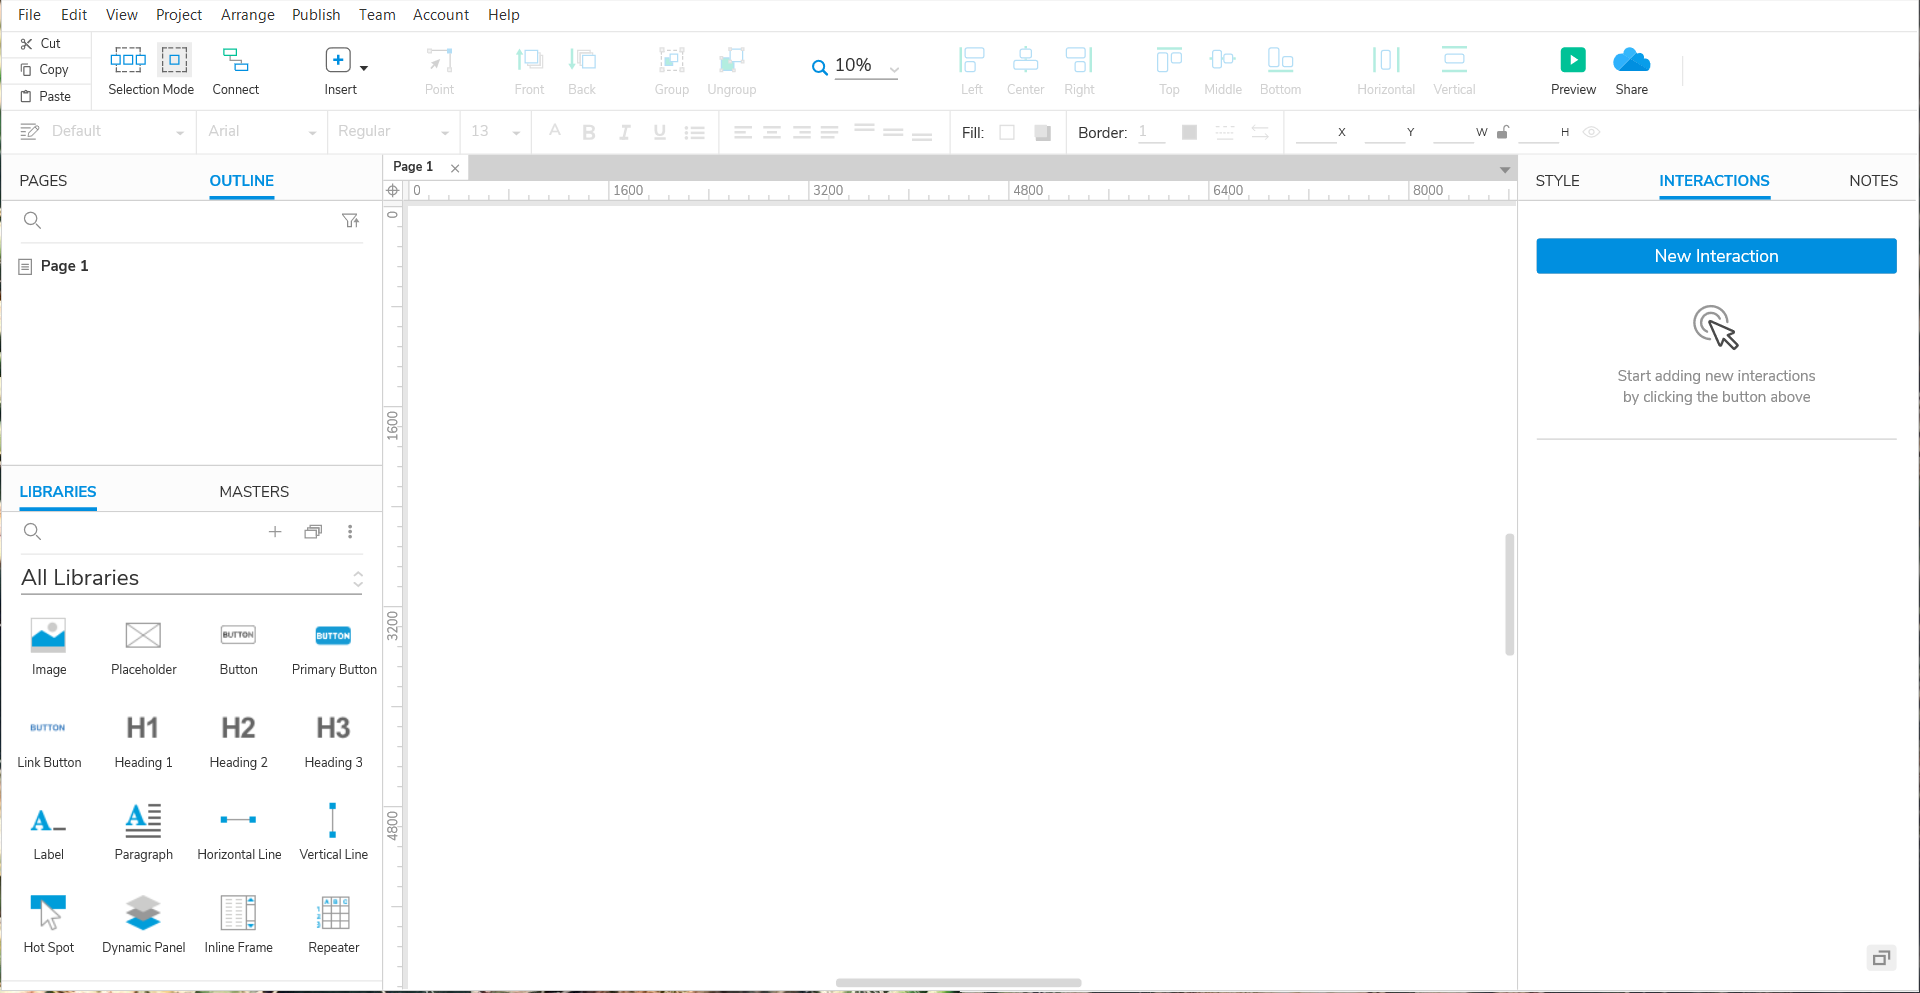
\includegraphics[scale=0.4]{figures/Axure_Full.png}
  \captionof{figure}{Axure RP 9}
  \label{fig:Axure_Full}
\end{center}

In den mittig platzierten Workspace können Elemente aus den Libraries links oder eigene, externe Elemente eingefügt werden.
Zieht man nun beispielsweise eine Droplist und drei Kreiselemente aus den Libraries links in den Workspace passt sich die Outline wie in \cref{fig:Axure_Outline} zu sehen entsprechend an.
Mithilfe dieser Outline kann man innerhalb des Projektes navigieren, was vor allem praktisch ist wenn sich mehrere Elemente, wie auch in diesem Beispiel zu sehen, überlagern.
Elemente lassen sich auch zu Dynamic Panels gruppieren, was vor allem dann nötig ist wenn man ein Drag und Drop Verhalten simulieren möchte, da dies die einzigen Widgets sind die dieses Verhalten unterstützen.

\begin{center}
  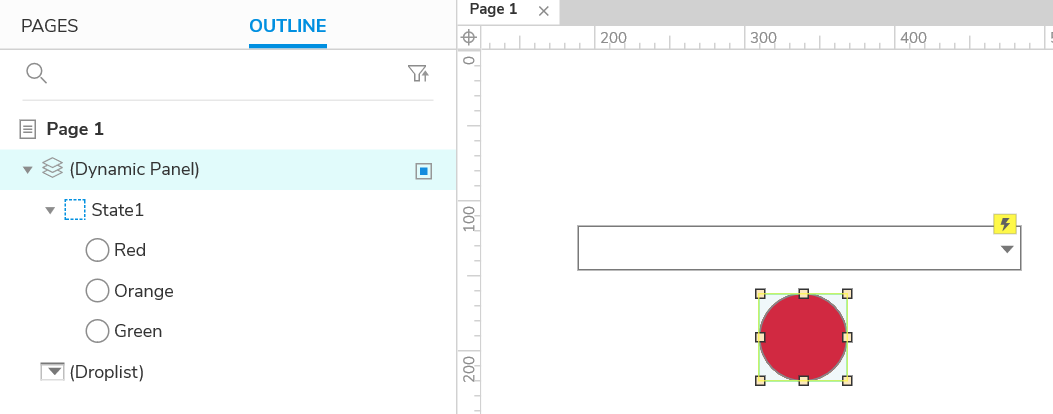
\includegraphics[scale=0.4]{figures/AXURE_Outline.PNG}
  \captionof{figure}{Axure RP 9 Outline}
  \label{fig:Axure_Outline}
\end{center}

Um den drei eingefügten Kreisen unterschiedliche Farben zuzuweisen ist es nötig deren Properties zu bearbeiten.
Die ist in AXURE RP über das Stlye Panel möglich, welches in \cref{fig:Axure_Style} zu sehen ist.
Hier ist es beispielsweise ebenfalls möglich Skalierungen vorzunehmen, oder Umrandungen und Schatten hinzuzufügen.

\begin{center}
  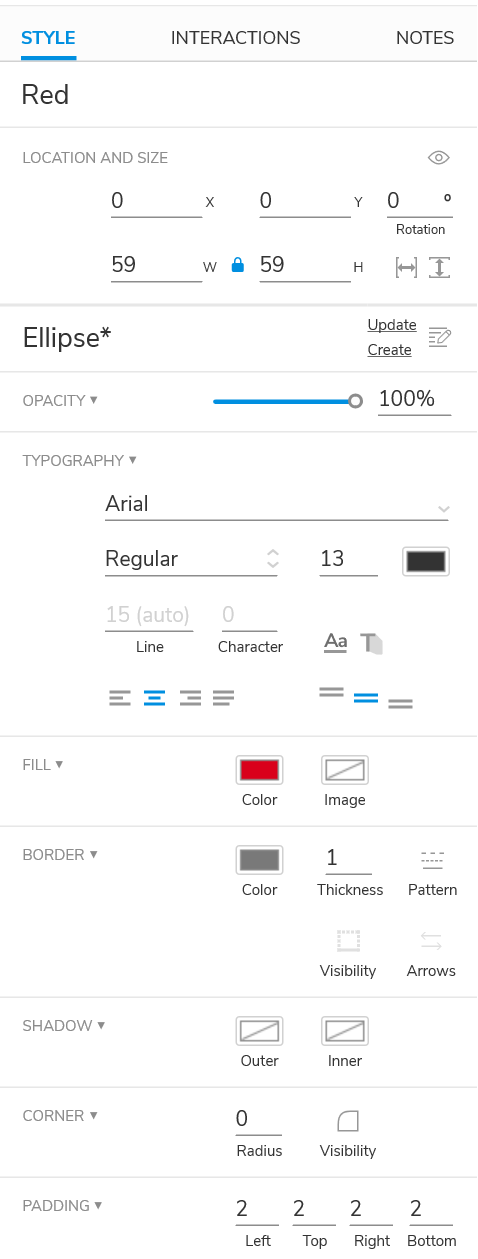
\includegraphics[scale=0.4]{figures/AXURE_Style.PNG}
  \captionof{figure}{Axure RP 9 Style Properties}
  \label{fig:Axure_Style}
\end{center}

Wenn man nun erreichen möchte, das die Farbe des sichtbaren Kreises ich an der Auswahl innerhalb der Droplist orientiert muss Logik zu dem Prototypen hinzugefügt werden.
Zuerst ist es, wie in Teil a von \cref{fig:Droplist} zu sehen, nötig Optionen innerhalb der Droplist hinzuzufügen.
Innerhalb des Interactionpanels besteht dann die Möglichkeit, über IF Conditions abzufragen, welche Option aktuell ausgewählt ist und die Visibility der Kreise entsprechend zu regulieren.

\begin{figure}%
\centering
\subfloat[][]{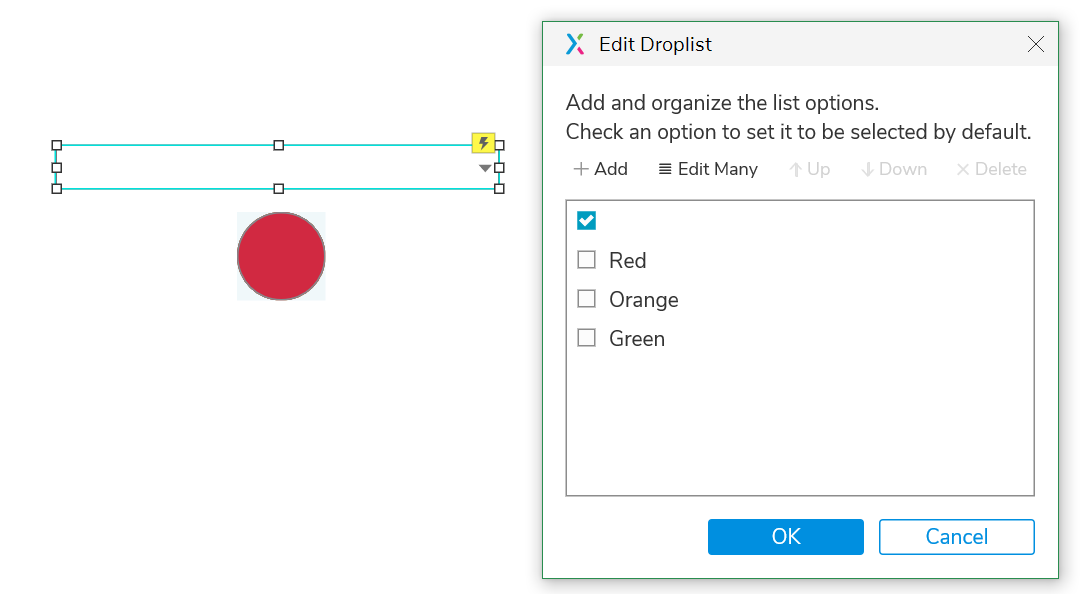
\includegraphics[width=0.5\linewidth]{figures/AXURE_Droplist.PNG}}%
\qquad
\subfloat[][]{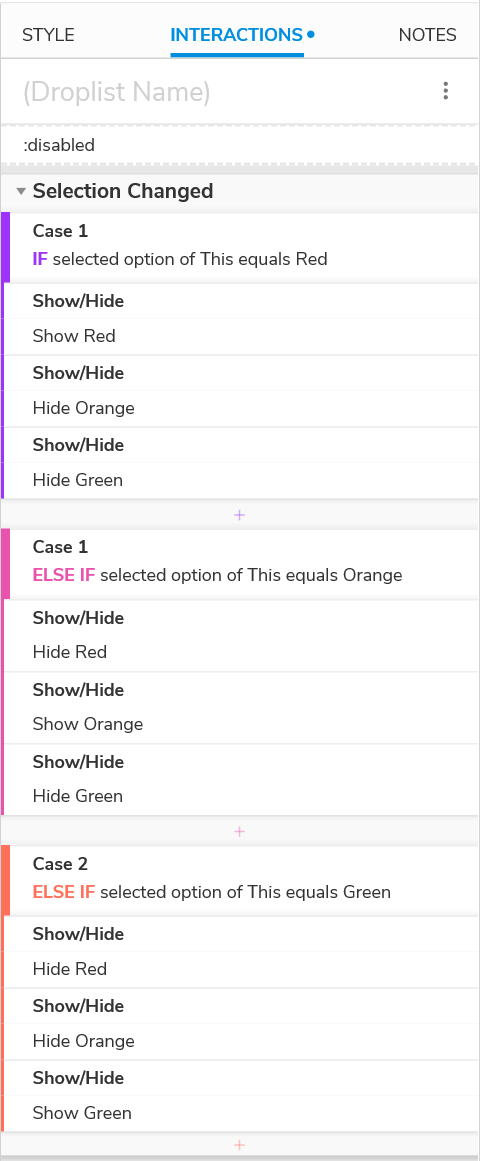
\includegraphics[width=0.3\linewidth]{figures/AXURE_Droplist_Conditions.PNG}}%

\caption{AXURE RP Droplist und Conditions}%
\label{fig:Droplist}
\end{figure}

Hat man die Modellierung abgeschlossen, oder möchte etwas überprüfen, bietet AXURE RP die Möglichkeit einer lokalen Preview.
Diese verhält sich exakt so, wie sich der abgeschlossene Prototyp ebenfalls verhalten wird und eignet sich deshalb gut für selbständige Validierung der bisherigen Umsetzung.
Testet man das soeben modellierte Beispiel in der Preview sieht man in \cref{fig:Droplist} , dass sich die Farbe des Kreises, wie gewünscht, immer an die Auswahl der Droplist anpasst.
\begin{figure}%
\centering
\subfloat[][]{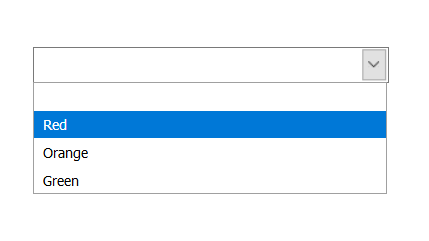
\includegraphics[width=0.3\linewidth]{figures/AXURE_red.PNG}}%
\qquad
\subfloat[][]{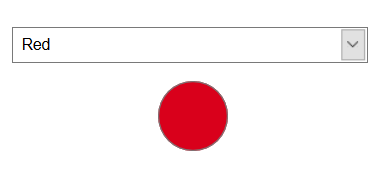
\includegraphics[width=0.3\linewidth]{figures/AXURE_red02.PNG}}%
\qquad
\subfloat[][]{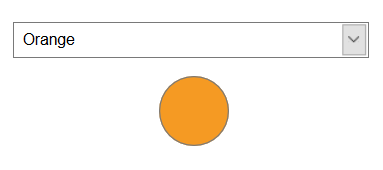
\includegraphics[width=0.3\linewidth]{figures/AXURE_orange.PNG}}%
\qquad
\subfloat[][]{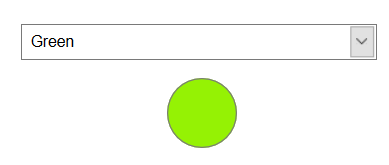
\includegraphics[width=0.3\linewidth]{figures/AXURE_green.PNG}}%

\caption{AXURE RP Preview}%
\label{fig:Preview}
\end{figure}

Ist die Modellierungsarbeit beendet bietet AXURE RP die Möglichkeit, dass Projekt in die AXURE CLOUD zu laden.
Hier können andere Mitarbeiter über einen generierten Link auf das funktionale Endprodukt zugreifen, ohne das eigentliche Projekt sehen oder bearbeiten zu können.
Dadurch ist es nun einerseits möglich andere UX Designer Funktionalitäten des Prototypen testen zu lassen, wobei sie auch an den entsprechenden Stellen Kommentare und TODO's hinterlassen können.
Außerdem besteht durch den Link die Möglichkeit den Prototypen für die Testpersonen im Rahmen des Usability Tests zugänglich zu machen.

\subsection{Interaktionsmöglichkeiten}

Im dritten Schritt des Human-centered design process ist es die Aufgabe des Interaction Designers die Interaktionsmöglichkeiten zu spezifizieren.
Dies ist deshalb notwendig, da es gerade bei Prototypen die ein komplexes System simulieren sollen, nicht möglich oder nötig ist alle Funktionen des Systems zu simulieren.
Daher wird vor der Erstellung des Prototyps festgelegt welche Interaktionen von den Nutzern durchführbar sein müssen um die geplanten Verbesserungen validieren zu können.

Für die Überprüfung der Usability der Ergänzungen ist es jedoch nicht ausreichend nur die neuen oder ergänzten Funktionen zu simulieren.
Um diese Ergänzungen überhaupt anwenden zu können muss der Nutzer einen gewissen Punkt innerhalb des Modellierungsprozesses erreicht haben.
Um an diesen Punkt zu gelangen ist es unbedingt notwendig, dass dem Nutzer gewissen Grundfunktionen von EB Guide zur Verfügung stehen.
Das bedeutet konkret, dass es für den Nutzer möglich sein muss wie gewohnt Elemente per Drag and Drop in den View zu ziehen, und diese dort auch frei bewegen zu können.
Ebenfalls müssen die Properties dieser Elemente angepasst werden können und die Elemente müssen wie gewohnt auf die Eingaben des Nutzers reagieren.
Das sich die Funktionen \glqq publish to template interface\grqq{} innerhalb der Templates befindet, muss es auch die Möglichkeit bestehen Templates anzulegen.

Darauf aufbauend müssen noch die neuen oder veränderten Funktionen in den Prototypen integriert werden.
Dazu zählt konkret, dass die Funktion \glqq publish to template interface\grqq{} verlagert wird und die alte Möglichkeit dafür vorerst nicht simuliert werden muss.
Zusätzlich muss es nun möglich sein mehrere Elemente gleichzeitig auszuwählen und hierfür ein Propertiepanel einzublenden.
Die Anpassung der Properties müssen sich in diesem Fall auch auf alle angewählten Elemente auswirken, und diese müssen auch gemeinsam im View bewegt werden können.
Zusätzlich müssen noch die neuen Alignment Actions, sowie die Funktion Insert in Template angezeigt werden und ausführbar sein.

\subsection{Vorgehensweise}

Viel Arbeiten mit Screenshots aus EB Guide
Funktionlität auf das nötigste beschränken

\section {Implementierung Filter}
\subsection {Zielsetzung}
Optische und Funktionale Umsetzung des UX Design

\subsection {Projektaufbau}

Model-View-ViewModel (MVVM) 
\cite{.g}

CollectionViewSource
\cite{dotnetbot.}

\subsection {Vorgehensweise}

CollectionViewSource.Filter
\cite{dotnetbot.b}

\lstinputlisting[language=Python ,caption={Widget Properties Filter},captionpos=b]{listings/Filter.cs}

\lstinputlisting[language=Python ,caption={Filter Constructor},captionpos=b]{listings/Filter_Constructor.cs}

\lstinputlisting[language=Python ,caption={CollectionViewSource()},captionpos=b]{listings/ICollectionView.cs}

\lstinputlisting[language=XML,caption={Filterpanel in xaml},captionpos=b]{listings/Filter_Panel.xaml}


